%!TEX root = ../my_thesis.tex
\chapter{Implémentation logicielle des algorithmes de décodage à Liste} % (fold)

% Intro chapitre

\vspace*{\fill}
\minitocTITI
\vspace*{\fill}
\newpage


\section*{Introduction}

\begin{figure}[t]
  \centering
  \subfloat[Stations de bases traditionnelle]{
  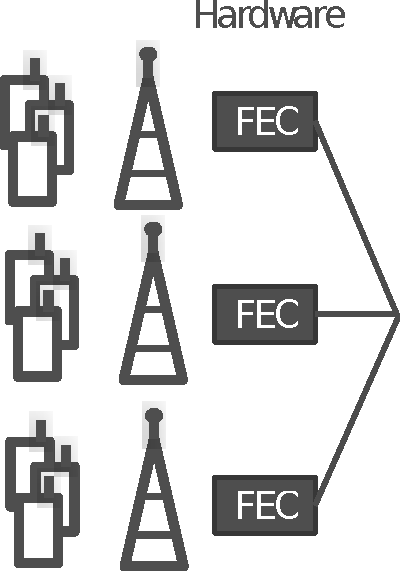
\includegraphics[scale=0.5]{main/ch2_fig/bs}
  \label{fig:bs}
  }
  \quad\quad
  \subfloat[Séparation BBU / RF]{
  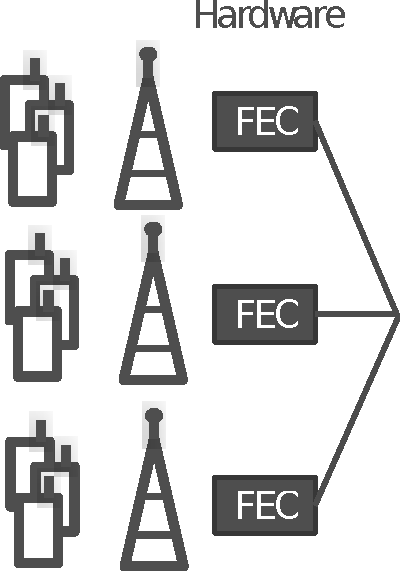
\includegraphics[scale=0.5]{main/ch2_fig/bs}
  \label{fig:bbu}
  }
  \quad\quad
  \subfloat[Cloud-RAN]{
  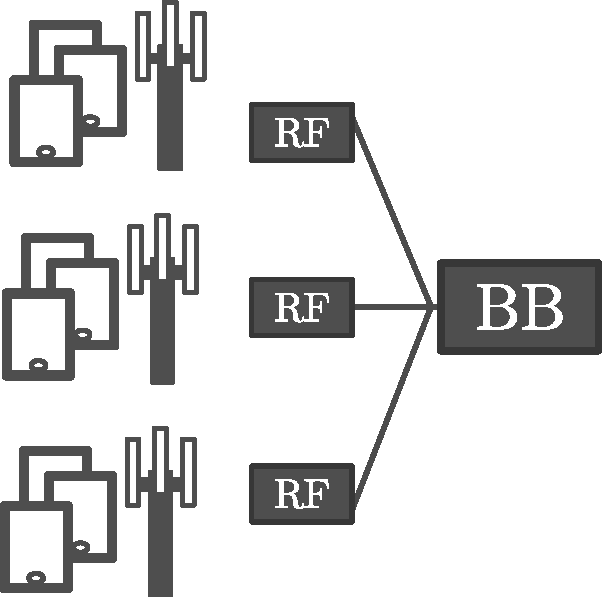
\includegraphics[scale=0.5]{main/ch2_fig/c-ran}
  \label{fig:c-ran}
  }
  \caption{\'Evolution de l'architecture des stations de base}
  \label{fig:bs_evo}
\end{figure}

La virtualisation des réseaux radio mobiles est considérée par les acteurs industriels \cite{ericsson_cloud_2015,huawei_5g:_2013,checko_cloud_2015} comme académiques \cite{wubben_benefits_2014,rost_cloud_2014} comme une fonctionnalité prometteuse. Elle est illustrée en Figure~\ref{fig:bs_evo}. Dans les premières génération, 1G et 2G illustrées en Figure \ref{fig:bs}, toutes les étapes de traitement du signal sont réalisées dans la station de base, à proximité de l'antenne, comme montré en Figure~\ref{fig:bs}. Une première évolution introduite dans les réseaux 3G est la séparation des traitements en bande de base (BBU : Base Band Unit) d'un coté et des traitements fréquence radio (RF : radio frequency) de l'autre. Comme représenté en Figure~\ref{fig:bbu} tandis que la BBU, distante de l'antenne, s'occupe du traitement en bande de base, dont le codage canal, la cellule RF a uniquement pour rôle la conversion du signal en signal RF. L'avantage de cette évolution est de pouvoir placer les stations BBU plus proches des centres urbains pour faciliter la maintenance.

L'étape suivante est nommée Cloud-RAN (Cloud Radio Access Network). Un groupe de BBUs est alors partagé entre plusieurs antennes et des optimisations entre BBUs peuvent être envisagées. Ces optimisations doivent permettre i) une meilleure adaptabilité aux traffics non uniformes, ii) des économie d'énergie, iii) des augmentations de débits et des réductions de la latence et enfin iv) de meilleures évolutivités et maintenabilité. Pour cela, ces BBUs doivent être virtualisées. Il ne doit plus y avoir un support matériel unique pour chaque BBU, mais au contraire, les calculs doivent être distribué sur le Cloud. Pour que cela soit réalisable, il est nécessaires que tous les algorithmes exécutés par les BBUs soient implémentés logiciellement. Or le décodage canal est une des tâches les plus intensives en calcul de l'ensemble des traitements en bande de base \cite{rodriguez_towards_2017,nikaein_processing_2015}. Ainsi, des implémentations efficaces et flexibles de codes correcteurs d'erreurs, comme celles présentées dans ce chapitre, sont nécessaires.

Ce chapitre est divisé comme suit. Tout d'abord, l'état de l'art des implémentations logicielles des algorithmes SC et SCL sur des processeurs à usage général est présenté dans la Section~\ref{sec:art_scl}. Les principales techniques permettant d'atteindre de hauts débits et de faibles latences sont détaillées. Un effort particulier a été réalisé afin de rendre les implémentations proposées génériques et flexibles. Dans un souci de clarté, les concepts de généricité et de flexibilité sont définis précisément et leurs implications sont détaillées dans la Section~\ref{sec:gen_scl}. Pour atteindre des débits et des latences compétitifs, des optimisations d'implémentations ont été proposées et sont décrites en Section \ref{sec:opti_scl}. Enfin, en Section~\ref{sec:exp_scl} les implémentations proposées sont comparées entre elles et avec l'état de l'art.

\section{\'Etat de l'art des implémentations logicielles d'algorithmes de décodage de codes polaires}
\label{sec:art_scl}

\subsection{Vectorisation}
Les processeurs à usage général (GPPs : General Purpose Processors) modernes sont de manière générale équipés d'unités de calcul vectoriel SIMD (Single Instruction Mutiple Data). Les architectures de processeurs x64 définissent par exemple des jeux d'instructions SIMD allant jusqu'à des tailles de 256 bits. Ces instruction incluent des opérations de chargement, sauvegarde et de mélange afin d'accéder aux données en mémoire et de les déplacer à des endroits voulus dans le registre, ainsi que des opérations de calcul, comme les additions, soustraction, multiplication.

Réduire le temps de décodage des algorithmes de décodage de codes polaires est une technique classique utilisée dans de nombreuses implémentations pour l'algorithme SC \cite{giard_fast_2014,giard_low-latency_2016,sarkis_fast_2014,sarkis_autogenerating_2014,giard_low-latency_2016,gal_software_2014,cassagne_efficient_2015,cassagne_energy_2016} comme pour l'algorithme SCL \cite{sarkis_increasing_2014,sarkis_fast_2016,shen_low-latency_2016}. Dans nos travaux est utilisée une librairie générique et portable implémentant les fonctions élémentaires des codes polaires \cite{cassagne_efficient_2015}. Elle est basée elle-même sur la librairie MIPP \cite{cassagne2018mipp} qui est une encapsulation des instructions SIMD dont la description logicielle est écrite dans le langage C++.

  \lstset{linewidth=0.7\textwidth, xleftmargin=0.025\textwidth, xrightmargin=0.05\textwidth}

  \begin{figure}[t]
  \begin{lstlisting}[language=C++, numbers=left, numbersep=0.3em, tabsize=2, basicstyle=\footnotesize\ttfamily]
class API_polar
{
  template <typename R>
  mipp::Reg<R> f_simd(const mipp::Reg<R> &la,
                      const mipp::Reg<R> &lb)
  {
    auto abs_la  = mipp::abs(la);
    auto abs_lb  = mipp::abs(lb);
    auto abs_min = mipp::min(abs_la, abs_lb);
    auto sign    = mipp::sign(la, lb);
    auto lc      = mipp::neg(abs_min, sign);

    return lc;
  }

  template <typename B, typename R>
  mipp::Reg<R> g_simd(const mipp::Reg<R> &la,
                      const mipp::Reg<R> &lb,
                      const mipp::Reg<B> &sa)
  {
    auto neg_la = mipp::neg(la, sa);
    auto lc     = neg_la + lb;

    return lc;
  }

  template <typename B>
  mipp::Reg<B> h_simd(const mipp::Reg<B>& sa,
                      const mipp::Reg<B>& sb)
  {
    return sa ^ sb;
  }
};
  \end{lstlisting}
  \caption{Implémentation des fonctions $f$, $g$ et $h$ utilisant la librairie MIPP.}
  \label{fig:mipp}
  \end{figure}
L'utilisation de cette librairie présente plusieurs avantages. Premièrement le code source apparaît clair, lisible et compact, contrairement à ce qui serait obtenu en utilisant le langage assembleur. Un extrait du code est donné en Figure~\ref{fig:mipp}. Deuxièmement, ce code source est portable. En effet, le code ainsi obtenu est compatibles avec différentes cibles matérielles (Intel x86, Xeon KNL et ARM) et il est possible d'utiliser différents jeux d'instructions (SSE, AVX, AVX-512, NEON). Troisièmement, plusieurs formats de représentation des données réelles sont utilisable : virgule flottante sur des mots de 32 bits, virgule fixe sur des mots de 8 ou 16 bits. Cette versatilité est obtenue sans perte de performance comme démontré dans \cite{cassagne2018mipp}.

Dans le contexte du décodage de codes polaires comme évoqué en Section \ref{subsubsec:parallel}, il existe deux stratégies principales afin d'utiliser le parallélisme SIMD. Les éléments d'un registre sont utilisés soit pour décoder de multiples trames en parallèle (\textit{inter-trame}), soit pour accélérer le décodage de chaque trame prise individuellement (\textit{intra-trame}). Dans les travaux présentés ici, seuls la stratégie \textit{intra-trame} est utilisée. L'avantage de cette technique est une latence inférieure. Le principe est d'utiliser le parallélisme disponible grâce aux fonctions $f$, $g$ et $h$ qui peuvent être effectués simultanément sur les \noeuds de grande taille, donc en haut de l'arbre, comme précisé toujours en Section \ref{subsubsec:parallel}. Il est également possible d'utiliser des instructions SIMD pour réaliser les opérations sur les feuilles. En effet, que ce soit dans les feuilles de type \texttt{R1}, \texttt{REP} ou \texttt{SPC}, il est nécessaire d'effectuer des opérations de seuillage sur un nombre de LLRs correspondant à la taille du \noeud. Ce seuillage est effectué parallèlement sur chacun de ces LLRs grâce à des instructions SIMD.

Toutefois, le parallélisme n'est utilisable que dans la partie supérieure de l'arbre, lorsque les \noeuds sont de tailles supérieure au parallélisme des unités SIMD. Dans le bas de l'arbre, près des feuilles, la librairie polaire \cite{cassagne_efficient_2015} utilise automatiquement les versions séquentielles des implémentations des fonctions élémentaires. Dans le cas de l'algorithme CASCL sur un code polaire de taille (2048, 1723) permet une augmentation du débit d'environ 20\%.


\subsection{Déroulage}
\label{subsec:unroll}
Une deuxième technique utilisée dans les travaux récents est le déroulage du code source \cite{sarkis_autogenerating_2014,giard_fast_2014,cassagne_efficient_2015,cassagne_energy_2016}. Il découle de l'observation faite sur les décodeurs de l'algorithme SC qu'un temps non négligeable est passé lors de différents tests au cours du parcours de l'arbre. Or il est possible d'éviter ces tests en générant un code source déroulé avant la compilation. Une illustration de ce déroulage est donnée en Figure~\ref{fig:unrolling}. D'un coté, dans le code non déroulé en Figure \ref{fig:alg_rolled}, des appels récursifs de la fonction \textit{DecodeNode} sont réalisés, qui peuvent être coûteux. De plus, des tests doivent être réalisé pour détecter le rendement de chaque feuille afin d'appliquer les fonctions \texttt{R0} ou \texttt{R1}. Au contraire, dans l'implémentation décrite en Figure~\ref{fig:alg_unrolled}, aucun appel récursif n'est réalisé, aucun test non plus. Seul les fonctions élémentaires polaires sont appelées.

De plus, l'arbre de décodage que nous prenons en exemple, en Figure~\ref{fig:unrolled_tree}, n'est pas élagué. Lorsque l'on ajoute l'élagage, le nombre de tests effectués au cours du parcours de l'arbre augmente en proportion du nombre total d'instructions, car le nombre de fonctions polaires différentes augmente. En effet, les fonctions \texttt{REP} et \texttt{SPC} sont ajoutées ainsi que des versions différentes des fonction $f$, $g$ et $h$ prenant en compte l'existence des \noeuds spécialisés de l'arbre élagué, comme décrit dans \cite{sarkis_fast_2014,cassagne_efficient_2015}. Dans certains cas, le déroulage du code source permet d'augmenter jusqu'à un facteur 2 les débits de décodage \cite{sarkis_autogenerating_2014}. La technique de déroulage a été également adaptée pour l'algorithme SCL \cite{sarkis_fast_2016}.

  \begin{figure}[t]
  \subfloat[Code non déroulé.]{
  \begin{minipage}{.35\linewidth}
  	\LinesNumberedHidden
    \begin{algorithm}[H]
      \SetAlgoLined
      \textit{DecodeNode}($\mathcal{N}_{0,0}$)\;
	  \SetKwProg{Fn}{Function}{}{}
	  \Fn{DecodeNode ($\mathcal{N}_{i,j}$)}{
	    \eIf{i<n}
	    {
	     $f(\mathcal{N}_{i,j})$\;
	     \textit{DecodeNode}($\mathcal{N}_{i+1,2j}$) \;
	     $g(\mathcal{N}_{i,j})$\;
	     \textit{DecodeNode}($\mathcal{N}_{i+1,2j+1}$) \;
	     $h(\mathcal{N}_{i,j})$\;
	    }
	    {
	      \eIf{$\mathcal{N}_{i,j}$\text est gelé}
	      {\texttt{R0}($\mathcal{N}_{i,j}$)\;}
	      {\texttt{R1}($\mathcal{N}_{i,j}$)\;}
	    }
      }
      \caption{Non Déroulé}%
    \end{algorithm}%
  \end{minipage}%
  \label{fig:alg_rolled}
  } 
  \quad\quad
  \subfloat[Code déroulé.]{
  \begin{minipage}{.16\linewidth}
    \LinesNumberedHidden
    \begin{algorithm}[H]
    \setstretch{1.045}
      \SetAlgoLined
	  $f(\mathcal{N}_{0,0})$\;
	  $f(\mathcal{N}_{1,0})$\;
	  \texttt{R0}($\mathcal{N}_{2,0}$)\;
	  $g(\mathcal{N}_{2,1})$\;
	  \texttt{R0}($\mathcal{N}_{2,1}$)\;
	  $h(\mathcal{N}_{1,0})$\;
	  $g(\mathcal{N}_{0,0})$\;
	  $f(\mathcal{N}_{1,1})$\;
	  \texttt{R1}($\mathcal{N}_{2,2}$)\;
	  $g(\mathcal{N}_{1,1})$\;
	  \texttt{R1}($\mathcal{N}_{2,3}$)\;
	  $h(\mathcal{N}_{1,1})$\;
	  $h(\mathcal{N}_{0,0})$\;
	  \mbox{}\\
      \caption{Déroulé}%
    \end{algorithm}%
  \end{minipage}%
  \label{fig:alg_unrolled}
  }
  \subfloat[Arbre décodé.]{
  \begin{minipage}{.35\linewidth}
  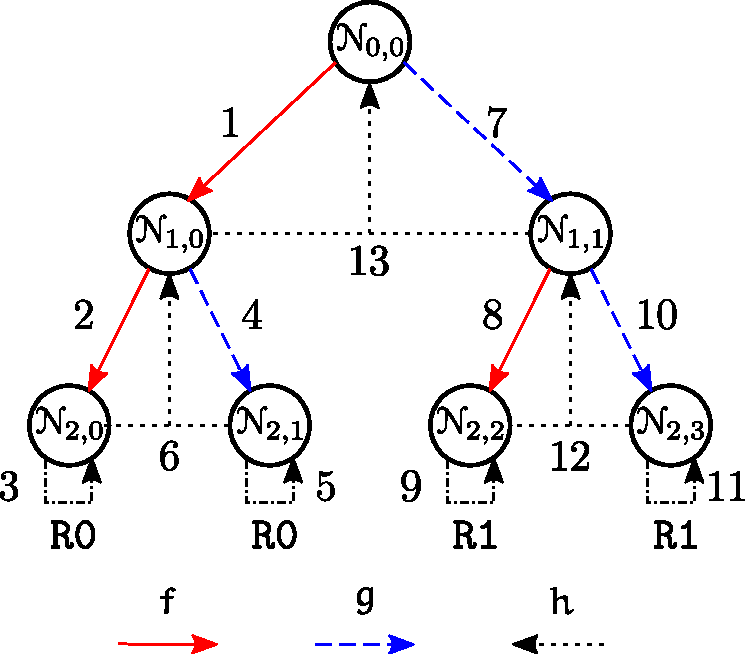
\includegraphics[width=\linewidth]{main/ch2_fig/unrolled_tree}
  \label{fig:unrolled_tree}
  \end{minipage}%
  }
  \caption{Déroulage du code source décrivant l'algorithme de décodage SC non élagué d'un code polaire (4,2) systématique.}
  \label{fig:unrolling}
\end{figure}

\subsection{Cibles}

\section{Généricité et Flexibilité d'un décodeur de codes polaire}

\label{sec:gen_scl}
\subsection{Définitions}
Les implémentations logicielles proposées sont génériques et flexibles. Afin d'éviter toute ambiguïté, ces termes doivent être définis précisément.
D'une part, le terme \textit{généricité} définit la capacité d'un décodeur à supporter n'importe quel encodage.
En effet, dans le contexte de télécommunications mobiles, les paramètres de l'encodeur changent constamment pour s'adapter au canal, en utilisant des méthodes adaptatives de modulation et de codage \cite{dahlman_4g:_2013} (AMC : Adaptive Modulation and Coding). Ainsi, les tailles de mot de code, les rendements, les ensembles de bits gelés évoluent. Des patrons de poinçonnage sont souvent nécessaires et des CRC sont concaténés pour détecter les erreurs et permettre des méthodes de transmission à demande de répétition automatique (ARQ : Automatic Repeat reQuest) ou leur équivalent hybride (HARQ : Hybrid ARQ). Un décodeur générique devra donc supporter toutes les combinaison possibles de chacun de ces paramètres.

D'autre part, le terme \textit{flexibilité} s'applique aux paramétrage de l'algorithme et des méthodes d'implémentation du décodeur, indépendamment du schéma d'encodage. Ces paramétrages-ci ne sont généralement pas imposés par le standard. Dans le cas de l'algorithme SCL, les paramètres suivants sont concernés : les variantes de l'algorithme (FASCL, PASCL), le format de quantification des données (virgule flottante ou fixe, nombre de bits), la taille de la liste $L$ ou encore l'élagage de l'arbre de décodage. La flexibilité du décodeur amène des degrés de liberté permettant des compromis entre pouvoir de correction, latence et débit, pour un schéma d'encodage donné.

Comme il sera détaillé dans les sections suivantes, tous les paramètres de généricité et de flexibilité cités sont pris en compte dans les décodeurs proposés. Ils sont déterminés par des fichiers de configurations, lus au moment de l'exécution. Aucune compilation n'est nécessaire en cas de changement de n'importe quel paramètre. De ce choix découle le fait que nous n'utilisons pas la technique de déroulage présentée en Section \ref{subsec:unroll}. En effet, cette technique implique la génération d'un code source pour chaque combinaison de paramètre différente. Ce

\subsection{Généricité}

\begin{figure}[t]
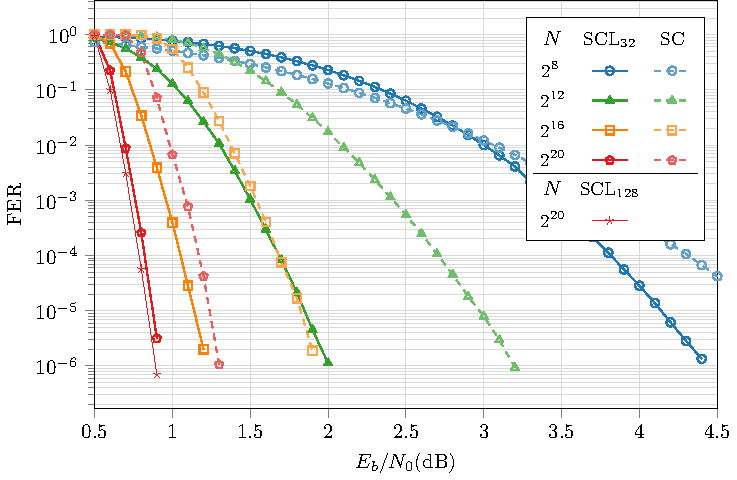
\includegraphics[width=\textwidth]{main/ch2_fig/curves/code/tikz/code}
\caption{Performances de décodage des algorithme SC et CASCL pour des tailles importantes de mots de code, $R=1/2$, CRC $c=32$ (GZip)}
\label{fig:large_scl}
\end{figure}

Les implémentations de décodeurs proposées gèrent n'importe quelle taille de mot de code. De plus, les débits des décodeurs étant compétitifs, il est possible d'explorer d'importantes tailles de mots de code ($N\geq2^{12}$) conjointement à des profondeurs de liste importante ($L \geq 32$), comme montré dans la Figure~\ref{fig:large_scl}. $N$ prend des valeurs allant de $2^8$ à $2^{20}$ et le rendement du code est $R=1/2$. Le CRC utilisé est défini dans le standard GZip, sa longueur est $c=32$ et son polunôme \texttt{0x04C11DB7}. Des simulations pour de telle valeurs de paramètres sont rares dans la littérature, et montrent que, bien que l'algorithme SCL ait été conçu pour améliorer les performances de décodage des codes polaires pour de petites tailles ($N<2^{12}$), son utilisation pour des codes de grande taille apporte également un important gain. Dans le cas où $N=2^{12}$, l'utilisation de l'algorithme CASCL avec une taille de liste $L=32$ amène un gain de d'environ 1.2 dB lorsque le FER est égal à $10^{-5}$. Ce gain diminue cependant lorsque $N$ augmente, avec 0.75 dB pour $N=2^{16}$ et 0.5 dB pour $N=2^{20}$. Des simulations ont également été réalisées pour une profondeur de liste $L=128$. Elles montrent que le gain par rapport à $L=32$ n'est pas significatif.

\subsection{Flexibilité}
Les paramètres de flexibilité sont eux aussi configuré lors de l'exécution du programme. Ils permettent des compromis divers entre la latence, le débit et les performance de correction. Ainsi, l'algorithme de décodage peut être ajusté finement pour un code polaire donné. Dans les sections à venir, ces paramètres de flexibilité sont détaillés et leurs effets analysés.

\subsubsection{Profondeur de la liste}
\begin{figure}[t]
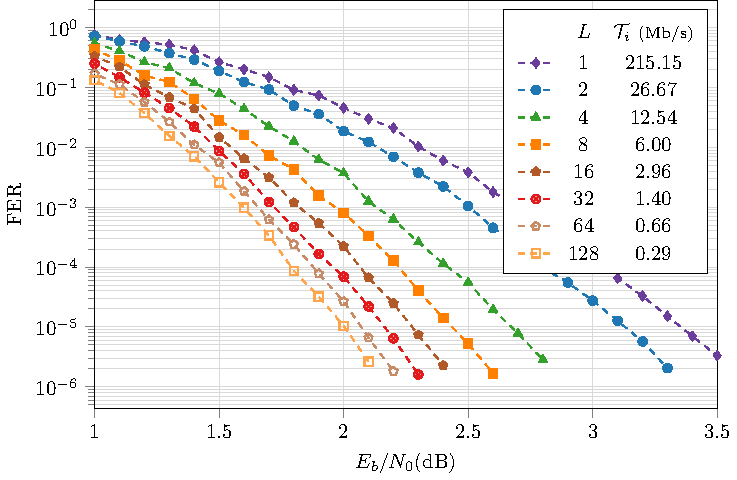
\includegraphics[width=\textwidth]{main/ch2_fig/curves/L/tikz/L}
\caption{Performances de décodage et débits de l'algorithme CASCL pour différentes valeurs de $L$ d'un code polaire ($2048,1024$) concaténé à un CRC $c=32$ (GZip).}
\label{fig:scl_l}
\end{figure}
La profondeur de la liste impacte directement le pouvoir de correction et la complexité de l'algorithme. En Figure~\ref{fig:scl_l} sont représentées les courbes de FER et les débits obtenus pour l'algorithme de décodage CASCL d'un code polaire ($2048$,$1024$). La complexité calculatoire augmente linéairement : le débit est approximativement doublé lorsque $L$ est doublé. Le seul cas ne respectant pas cette assomption est celui pour lequel $L=1$ qui correspond à l'algorithme SC, bien plus rapide puisque n'ayant pas à effectuer les calculs associés à l'algorithme SCL comme le tri, la génération des candidats, le calcul du CRC. Le FER évolue également avec $L$. \`A partir de $L\geq4$ et $E_b/N_0=2$, le FER est divisé par deux lorsque $L$ est doublé.

\subsubsection{Paramétrage fin de l'élagage}
L'élagage, tel que défini en Section~\ref{subsec:pruning} est paramétrable très finement dans les implémentations de décodeurs polaires proposées. Tout d'abord, chaque type de \noeud (\texttt{R0}, \texttt{R1}, \texttt{REP} et \texttt{SPC} peut être activé ou désactivé séparément. Cette capacité est utile pour explorer l'impact de l'utilisation de chaque \noeud sur le débit codé.

Il faut ici faire la distinction entre le débit codé  et le débit d'information. Soit $\mathcal{T}_F$, le nombre de trames décodées par seconde. Alors le débit d'information est $\mathcal{T}_i=K\mathcal{T}_F$, soit le nombre de bits d'informations décodés par seconde, et le débit codé est $\mathcal{T}_c=N\mathcal{T}_F$.

Pour explorer l'impact de l'utilisation des \noeuds sur le débit, il est  plus pertinent d'utiliser le débit codé. En effet, si l'on utilisait le débit d'information dans la Figure~\ref{fig:nodes}, le rendement du code biaiserait les débits : le débit des codes à haut rendement auraient un débit bien supérieurs aux codes à faibles rendement.
\begin{figure}[t]
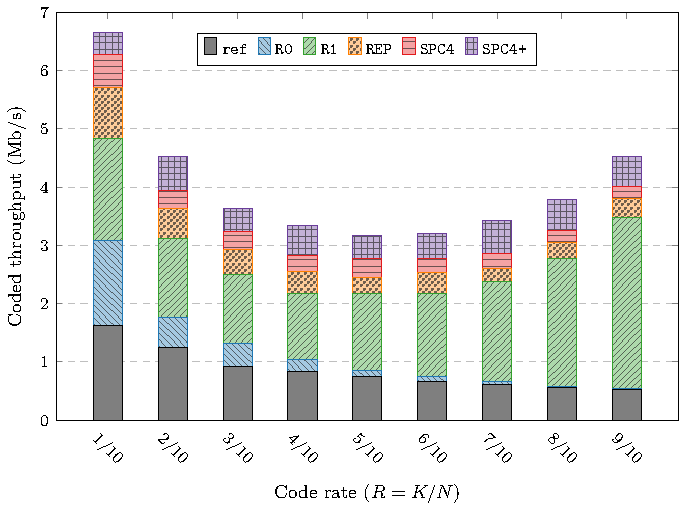
\includegraphics[width=\textwidth]{main/ch2_fig/curves/tree/tikz/tree}
\caption{Impact de l'activation des \noeuds d'élagage de l'algorithme CASCL, $N=2048$, $L=32$, $c=32$.}
\label{fig:nodes}
\end{figure}

\begin{figure}[t]
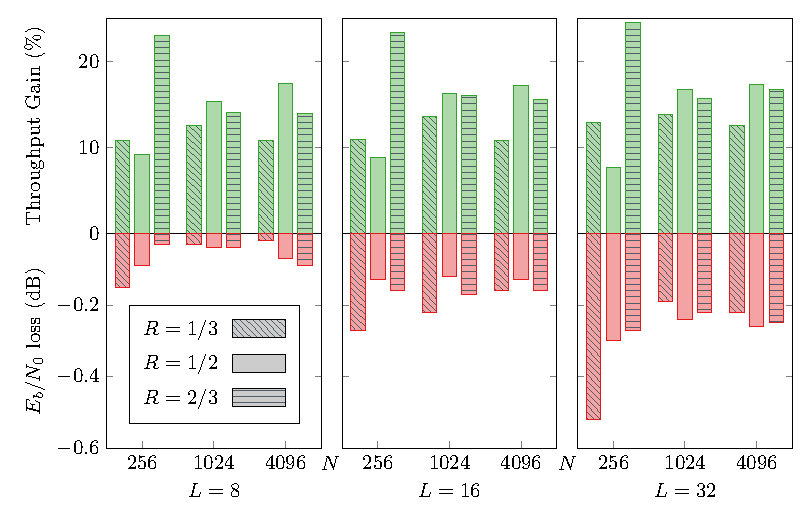
\includegraphics[width=\textwidth]{main/ch2_fig/curves/thr_spc/tikz/thr_spc_diff}
\caption{Effets de l'utilisation des \noeuds \texttt{SPC4+} dans l'algorithme CASCL à un FER de $10^{-5}$}
\label{fig:spc_impact}
\end{figure}

Le débit codé de l'algorithme non élagué (\texttt{ref}) diminue lorsque le rendement augmente. Cela s'explique par le fait que les feuilles de rendement 1, plus nombreuses dans les codes à hauts rendements, sont plus long à décoder que les feuilles de rendement 0. En effet, dans l'algorithme SCL, le traitement d'une feuille de rendement 0 correspond à la mise à jour de métriques, tandis que le traitement d'une feuille de rendement 1 correspond à la génération de candidats, la mise à jour de leurs métriques, le tri de celles-ci, et des duplications d'arbres de décodage.

Les aires hachurées en diagonales représentent l'amélioration des performances de décodage lorsque les \noeuds \texttt{R0} et \texttt{R1} de taille supérieures à un (c'est à dire les \noeuds plus haut que les feuilles) sont utilisés pour l'élagage. De manière attendue, l'élagage \texttt{R1} est plus efficace pour les codes à haut rendement et, inversement, l'élagage \texttt{R0} est plus efficace pour les codes à faible rendement. On observe la même tendance pour l'élagage des \noeuds \texttt{REP} plus efficace pour les codes de faibles rendements, qui en contiennent également beaucoup. La tendance est moins claire pour les \noeuds \texttt{SPC}.

Il fut également observé dans \cite{sarkis_fast_2014} que lorsque la taille des \noeuds \texttt{SPC} n'est pas limitée à 4, les performances de décodage peuvent être dégradées. Dans les implémentations proposées, le choix a été fait de donner la possibilité de paramétrer finement la taille des \noeuds activés pour chaque type de \noeuds. En conséquence, leur taille est limitée à 4 dans les aires labellisées \texttt{SPC4} dans la figure \ref{fig:nodes}. Les \noeuds \texttt{SPC4+} sont de tailles supérieures. 

Selon nos expérimentations, la dégradation des performances de correction due à l'utilisation des \noeuds \texttt{SPC4+} n'est pas systématique, dépendamment des caractéristique du code polaire considéré. La Figure\ref{fig:spc_impact}


\section{Optimisations de l'implémentation logicielle des décodeurs liste}
\label{sec:opti_scl}

\subsection{Algorithmes de tri}
\subsection{Accélération du contrôle de redondance cyclique}
\subsection{Gestion des sommes partielles}

\section{Expérimentations et mesures}
\label{sec:exp_scl}

\subsection{Comparaison des cibles}
\subsection{Comparaison des algorithmes}
\subsection{Comparaison avec l'état de l'art}
 
\section*{Conclusion}
